\documentclass{article}
\usepackage{tikz}
\usepackage{subfigure}

\begin{document}



\begin{figure}[h]
\centering 
    \subfigure{
        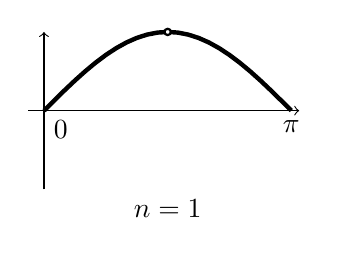
\begin{tikzpicture}[scale=1]
            \draw [->] (0,-1) -- (0,1);
            \draw [->] (-0.2,0) -- (pi+0.1,0);
            \draw[black, ultra thick, domain=0:pi] plot (\x, {sin(\x r)});
            \node [below right] at (0,0) {0};
            \node [below] at (pi,0) {$\pi$};
            \node [below] at (pi/2,-1) {$n=1$};
            \draw [black, thick, fill=white] (pi/2 ,1) circle [radius=0.04];
        \end{tikzpicture}
    }
    \subfigure{
        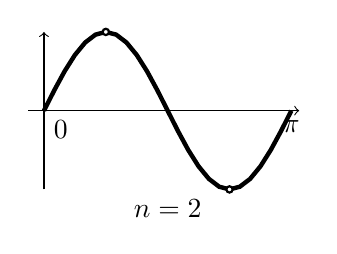
\begin{tikzpicture}[scale=1]
            \draw [->] (0,-1) -- (0,1);
            \draw [->] (-0.2,0) -- (pi+0.1,0);
            \draw[black, ultra thick, domain=0:pi] plot (\x, {sin(2*\x r)});
            \node [below right] at (0,0) {0};
            \node [below] at (pi,0) {$\pi$};
            \node [below] at (pi/2,-1) {$n=2$};
            \draw [black, thick, fill=white] (pi/4 ,1) circle [radius=0.04];
            \draw [black, thick, fill=white] (3*pi/4 ,-1) circle [radius=0.04];
        \end{tikzpicture}
    }
    \subfigure{
        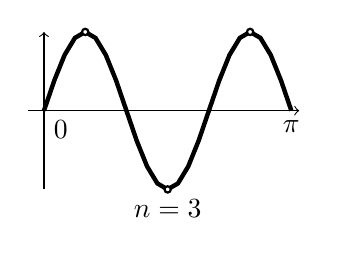
\begin{tikzpicture}[scale=1]
            \draw [->] (0,-1) -- (0,1);
            \draw [->] (-0.2,0) -- (pi+0.1,0);
            \draw[black, ultra thick, domain=0:pi] plot (\x, {sin(3*\x r)});
            \node [below right] at (0,0) {0};
            \node [below] at (pi,0) {$\pi$};
            \node [below] at (pi/2,-1) {$n=3$};
            \draw [black, thick, fill=white] (pi/6 ,1) circle [radius=0.04];
            \draw [black, thick, fill=white] (3*pi/6 ,-1) circle [radius=0.04];
            \draw [black, thick, fill=white] (5*pi/6 ,1) circle [radius=0.04];
        \end{tikzpicture}
     }
     \caption{}
\end{figure} 

\end{document}